%%%%%%%% ICML 2026 PAPER DRAFT %%%%%%%%%%%%%%%%%

\documentclass{article}

\usepackage[UTF8]{ctex}
\usepackage{microtype}
\usepackage{graphicx}
\usepackage{subcaption}
\usepackage{booktabs}
\usepackage{hyperref}
\usepackage[preprint]{icml2026}

\usepackage{amsmath}
\usepackage{amssymb}
\usepackage{mathtools}
\usepackage{amsthm}
\usepackage[capitalize,noabbrev]{cleveref}
\usepackage{tabularx}
\usepackage{array}
\usepackage[most]{tcolorbox}
\usepackage{ragged2e}
\usepackage{tikz}
\usetikzlibrary{arrows.meta,positioning,fit,backgrounds}

\newcommand{\system}{OpenFinance}
\newcommand{\tok}[1]{\nolinkurl{#1}}
\newcommand{\term}[1]{\mbox{\textsf{#1}}}
\newenvironment{tokenblock}{\begingroup\RaggedRight\setlength{\parfillskip}{0pt plus 1fil}}{\par\endgroup}
\newtcolorbox{verifybox}{
  colback=gray!6,
  colframe=gray!45,
  boxrule=0.5pt,
  arc=1.2pt,
  left=6pt,
  right=6pt,
  top=5pt,
  bottom=5pt,
  title={Where to verify},
  fonttitle=\bfseries,
  coltitle=black,
  colbacktitle=gray!14,
  enhanced,
  breakable
}

\hyphenpenalty=9000
\exhyphenpenalty=9000
\emergencystretch=1.2em
\hyphenation{OpenFinance Backtest EvidencePack FactorSpec FactorReport RobustnessReport counterfactual Orchestrator StrategyAgent BacktestRunner}

\definecolor{orchBlue}{HTML}{2F6DB3}
\definecolor{evidenceTeal}{HTML}{2C9C9A}
\definecolor{agentsPurple}{HTML}{7E5AA6}
\definecolor{artifactGray}{HTML}{6F7785}
\definecolor{riskAmber}{HTML}{C77D2B}
\definecolor{counterRed}{HTML}{C23B3B}

\icmltitlerunning{\smash{OpenFinance}}

\begin{document}

\twocolumn[
  \icmltitle{\system：面向量化研究与风控执行的\\可追踪多智能体工作台}

  \icmlsetsymbol{equal}{*}
  \begin{icmlauthorlist}
    \icmlauthor{MorikawaSōma}{m1}
  \end{icmlauthorlist}

  \icmlaffiliation{m1}{OpenFinance Project}
  \icmlcorrespondingauthor{MorikawaSōma}{morikawasoma@openfinance.dev}
  \icmlkeywords{multi-agent systems, quantitative finance, explainability, traceability}

  \vskip 0.3in
]

\printAffiliationsAndNotice{}

\begin{abstract}
本文给出 \system{} 的第三轮论文打磨稿，目标是让未读代码的读者也能完整回答四个问题：系统如何从提问跑到报告与风控；13 个智能体如何分工协作；因子与策略如何被构建、验证与选优；可解释性如何落实到可追溯、可复核、可回放。与前一轮相比，本文保留章节框架与 Figure 1/2 编号，重点修复排版卫生问题，并把方法部分改写为连续推导叙事：通过一个贯穿示例，把页面交互、后端阶段、产物对象与审计路径组织成可复述、可质疑、可复核的完整链路。
\end{abstract}

\section{引言}
量化研究系统的主要痛点通常不在单点模型能力，而在流程割裂：问题输入、证据检索、因子构建、策略评估、回测比较与风控审批分散在不同工具中，最终导致“结论可读但不可复核”。\system{} 将这些环节统一在 FastAPI + Next.js 的任务驱动架构中，并通过事件总线和注册中心形成可审计闭环 \cite{openfinance_repo}。

本文不强调“提出一个新模型”，而强调“给出一套可落地、可复盘的方法工程”。读者读完应能直接回答：
\begin{itemize}
  \item 系统从提问到风控是如何依次运行的；
  \item 13 个智能体谁负责什么、如何合并输出；
  \item 因子如何成为 \tok{FactorSpec} 并完成验证，策略如何由候选到选优；
  \item 在哪个页面、看哪些字段可以验证结论来源。
\end{itemize}

\section{项目总结框架}
\subsection{端到端运行流程}
\system{} 的 happy path 可以概括为：\textit{Question $\rightarrow$ Plan $\rightarrow$ Evidence $\rightarrow$ Factor $\rightarrow$ Strategy $\rightarrow$ Backtest $\rightarrow$ Report $\rightarrow$ Risk Gate}。

\begin{figure*}[t]
\centering
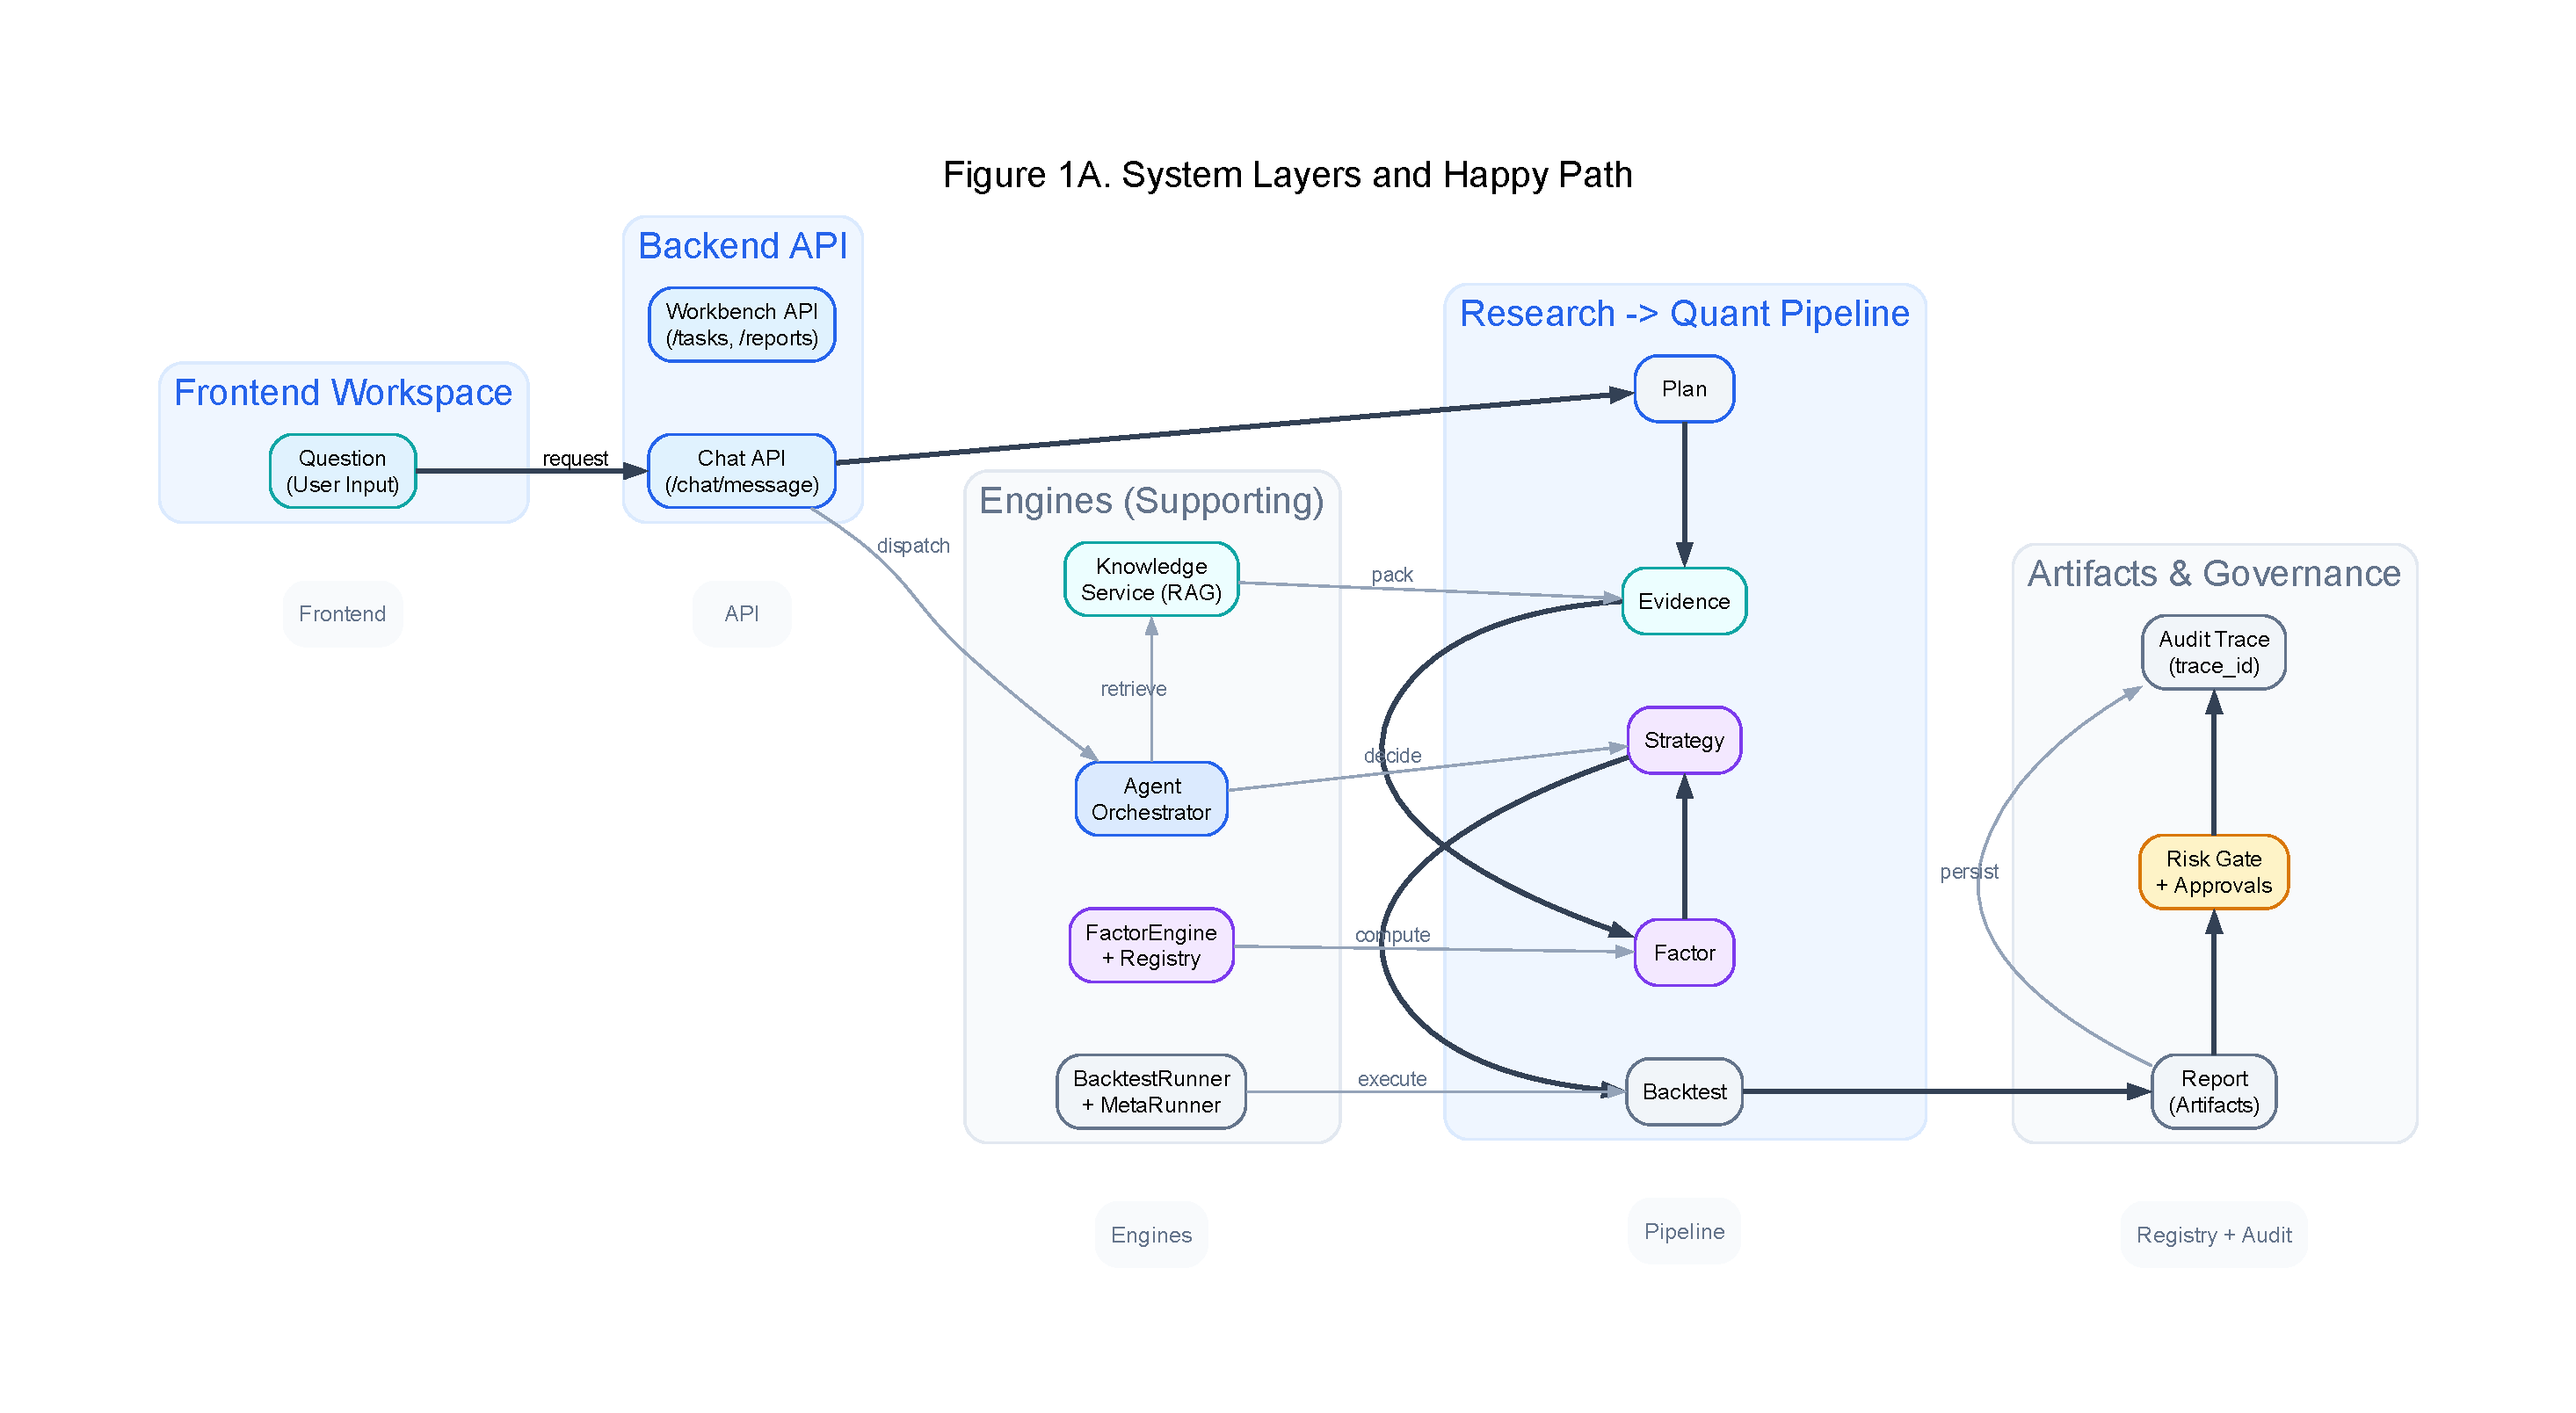
\includegraphics[width=\textwidth]{docs/figures/fig1a_system_layers.pdf}
\caption{System layers and end-to-end happy path. 图注（中文）：OpenFinance 的系统分层与端到端主线（Question $\rightarrow$ Plan $\rightarrow$ Evidence $\rightarrow$ Factor $\rightarrow$ Strategy $\rightarrow$ Backtest $\rightarrow$ Report $\rightarrow$ Risk Gate）。}
\label{fig:system-overview}
\end{figure*}

\subsection{贯穿示例（Worked Example）：从问题到报告的 10 步}
全篇统一使用一个示例：\textbf{“日经最近如何；基于当前 JP 市场给我一个低回撤策略并回测；再做高波动假设下的稳健性比较。”}

\begin{tokenblock}
\begin{enumerate}
  \item \textbf{意图定标（\tok{/chat}）}。系统先解决“目标函数到底是什么”的不确定性，把用户提问拆成回撤预算、市场边界和风险偏好三组约束。页面上会先出现约束标签，再生成 \tok{session_id} 与 \tok{intent_profile}，这一步决定后续选优是偏向稳健还是偏向收益弹性。

  \item \textbf{研究计划成形（\tok{/pipeline}）}。系统随后解决“要试哪些假设、何时停止”的不确定性，生成 \tok{plan_id} 及对应的阶段图。用户在 \tok{/pipeline} 看到的不是一句“开始回测”，而是可执行的实验矩阵与阶段完成条件，这让后续比较有统一刻度。

  \item \textbf{证据打包（\tok{/evidence}）}。此时要解决“结论是否有事实锚点”的不确定性，系统把检索到的材料压成 \tok{evidence_pack_id}。每条证据都有 \tok{source.title}、\tok{source.ts}、\tok{source.snippet} 和可信度字段，读者能在 Evidence 页直接区分“事实描述”和“策略解释”。

  \item \textbf{数据锁版（\tok{/tasks}）}。DataEngineer 对齐交易日历与字段口径，输出 \tok{dataset_version}，用来解决“是否发生时序错配或口径漂移”的不确定性。Tasks 页会出现 data-ready 阶段和版本号，后续所有报告都必须回指同一版本。

  \item \textbf{叙事转命题（\tok{/factors}）}。系统把“JP 市场波动抬升、流动性重定价”从叙事翻译成可检验命题，并给出首版 \tok{FactorSpec}。这一转换解决的是“研究语言能否变成可计算对象”的不确定性；没有这一步，因子只能靠文字复述，无法复现。

  \item \textbf{微型推导（证据 $\rightarrow$ 因子）}。在该示例里，\textit{volatility elevated} 与 \textit{liquidity repricing} 被映射成“防御型流动性调整动量”，并写成
  \[
  s_t=z(r_{20})-0.6\,z(v_{20})-0.4\,z(\ell_{20}) .
  \]
  其中 \(r_{20}\) 是 20 日收益，\(v_{20}\) 是 20 日实现波动，\(\ell_{20}\) 是 20 日流动性冲击代理。对应到系统对象时，\tok{inputs} 记录字段来源，\tok{transforms} 固化去极值与行业中性化，\tok{validation_plan} 指定 \tok{ic_mean}、\tok{decay}、\tok{oos_gap} 的门槛，\tok{failure_conditions} 和 \tok{cost_sensitivity} 则提前声明“什么情境下不该继续交易”。

  \item \textbf{因子体检（\tok{/reports/{runId}}）}。FactorEngine 先回答“这个信号是噪声还是真有方向性”，再决定是否进入策略层。用户在 Reports 页看到 \tok{ic_mean}、\tok{rank_ic_mean}、\tok{decay}、\tok{sensitivity} 后，可以判断它是“可预测且可交易”，还是“统计有效但交易上不可承受”。

  \item \textbf{候选策略生成（A/B）}。StrategyAgent 不直接给单一答案，而是把同一因子落成候选 A/B，并输出 \tok{tradeoff_summary} 与 \tok{why_not_selected}。这一步解决“同一信号如何在不同风险预算下落地”的不确定性，避免把选择过程藏在一段解释文字里。

  \item \textbf{回测账本与稳健性}。BacktestRunner 生成 \tok{run_id} 并保存 \tok{orders}、\tok{trades}、\tok{cost_breakdown}，随后由 \tok{RobustnessReport} 在高波动、成本翻倍和流动性恶化场景做矩阵比较。该示例里候选 B 在基准期收益略高，但在“成本$\times 2$”下回撤显著放大，因此排序被稳健性结果反转。

  \item \textbf{报告、门禁与回放（\tok{/risk}）}。最终报告把 \tok{factor_version}、\tok{strategy_version}、\tok{evidence_refs}、\tok{trace_id} 绑定在同一血缘链上，并进入 Risk Gate 审批。读者如果质疑“是否编故事”，可以通过 \url{/trace/\{trace_id\}/restore} 回放同一上下文，逐步核对证据、推理步骤和最终结论。
\end{enumerate}
\end{tokenblock}

\subsection{因子 $\rightarrow$ 策略 $\rightarrow$ 评估：前置机制解释}
\subsubsection{因子阶段：从“叙事”到“可检验命题”}
研究叙事天然含糊，例如“风险偏好下降”可以同时指向动量收缩、波动扩散或流动性折价。OpenFinance 的做法是先把叙事压缩成可检验命题，再把命题写入 \tok{FactorSpec}：字段定义了数据输入、变换链、验证门槛与失效情境，等价于给“因子成立”写了一份可执行契约。对于贯穿示例，这份契约明确要求信号既要在横截面上有方向（\tok{ic_mean} 为正），又不能在持有几天后快速蒸发（\tok{decay} 不能塌陷），否则它即使统计显著也不会进入交易层。

\subsubsection{策略阶段：从“信号有效”到“可交易决策”}
当因子通过体检后，系统并不会把它直接变成“唯一策略”，而是把同一信号在不同约束下展开成候选 A/B。A 通常收紧回撤和换手，B 通常提升信号响应速度；二者都继承同一份因子证据，却在交易成本、风格暴露和极端行情承受力上呈现不同轮廓。这样设计的关键是让 \tok{why_not_selected} 成为结构化产物，而不是事后解释，从而把“为什么不用另一个方案”纳入可审计对象。

\subsubsection{评估阶段：从“曲线漂亮”到“可复核结论”}
评估阶段的核心不是“谁的曲线更好看”，而是“谁在账本可实现、情境可承受、结论可复核”。因此系统同时保留 \tok{orders/trades} 账本、成本分解和稳健性矩阵：先确认收益是否来自可执行成交，再检查该收益是否依赖脆弱前提。贯穿示例中的候选 B 在基准样本略优，但在成本放大和波动抬升时迅速退化，最终被候选 A 反超，这也是本文强调“不是最大 Sharpe，而是约束下 Pareto 选优”的原因。

\subsection{前端页面协同机制}
系统并非“页面集合”，而是“工件视图集合”。同一 \tok{plan_id}、\tok{run_id}、\tok{trace_id} 在不同页面给出不同观察视角：Chat 看意图与推理、Pipeline 看阶段、Tasks 看状态机、Reports 看结果与归因、Evidence 看来源、Risk 看门控与审批。

\begin{verifybox}
\footnotesize
\begin{tabularx}{\linewidth}{@{}>{\bfseries}p{1.9cm}X@{}}
UI: & \tok{/chat}、\tok{/pipeline}、\tok{/tasks}、\tok{/reports}、\tok{/evidence}、\tok{/risk} \\
Artifacts: & \tok{plan_id}、\tok{evidence_pack_id}、\tok{factor_version}、\tok{strategy_version}、\tok{run_id}、\tok{trace_id} \\
Events: & \tok{task.created}、\tok{task.progress}、\tok{task.variant_started}、\tok{task.done} \\
\end{tabularx}
\end{verifybox}

\section{13 智能体架构与协作流程}
\subsection{角色分工}
13 个智能体分为两组：
\begin{itemize}
  \item \textbf{Research 6}：Buffett、Soros、Simons、Dalio、Kahneman、Factor，负责投资假设、反证挑战、因子有效性与市场解释；
  \item \textbf{Ops 7}：Librarian、DataEngineer、RiskManager、ExecutionTrader、ComplianceAudit、Strategy、Code，负责数据质量、执行约束、审计与实现可行性。
\end{itemize}
默认路径激活 Research 6；Ops 7 由 orchestrator 按任务场景按需激活。

\subsection{协作流程图}
\begin{figure*}[t]
\centering
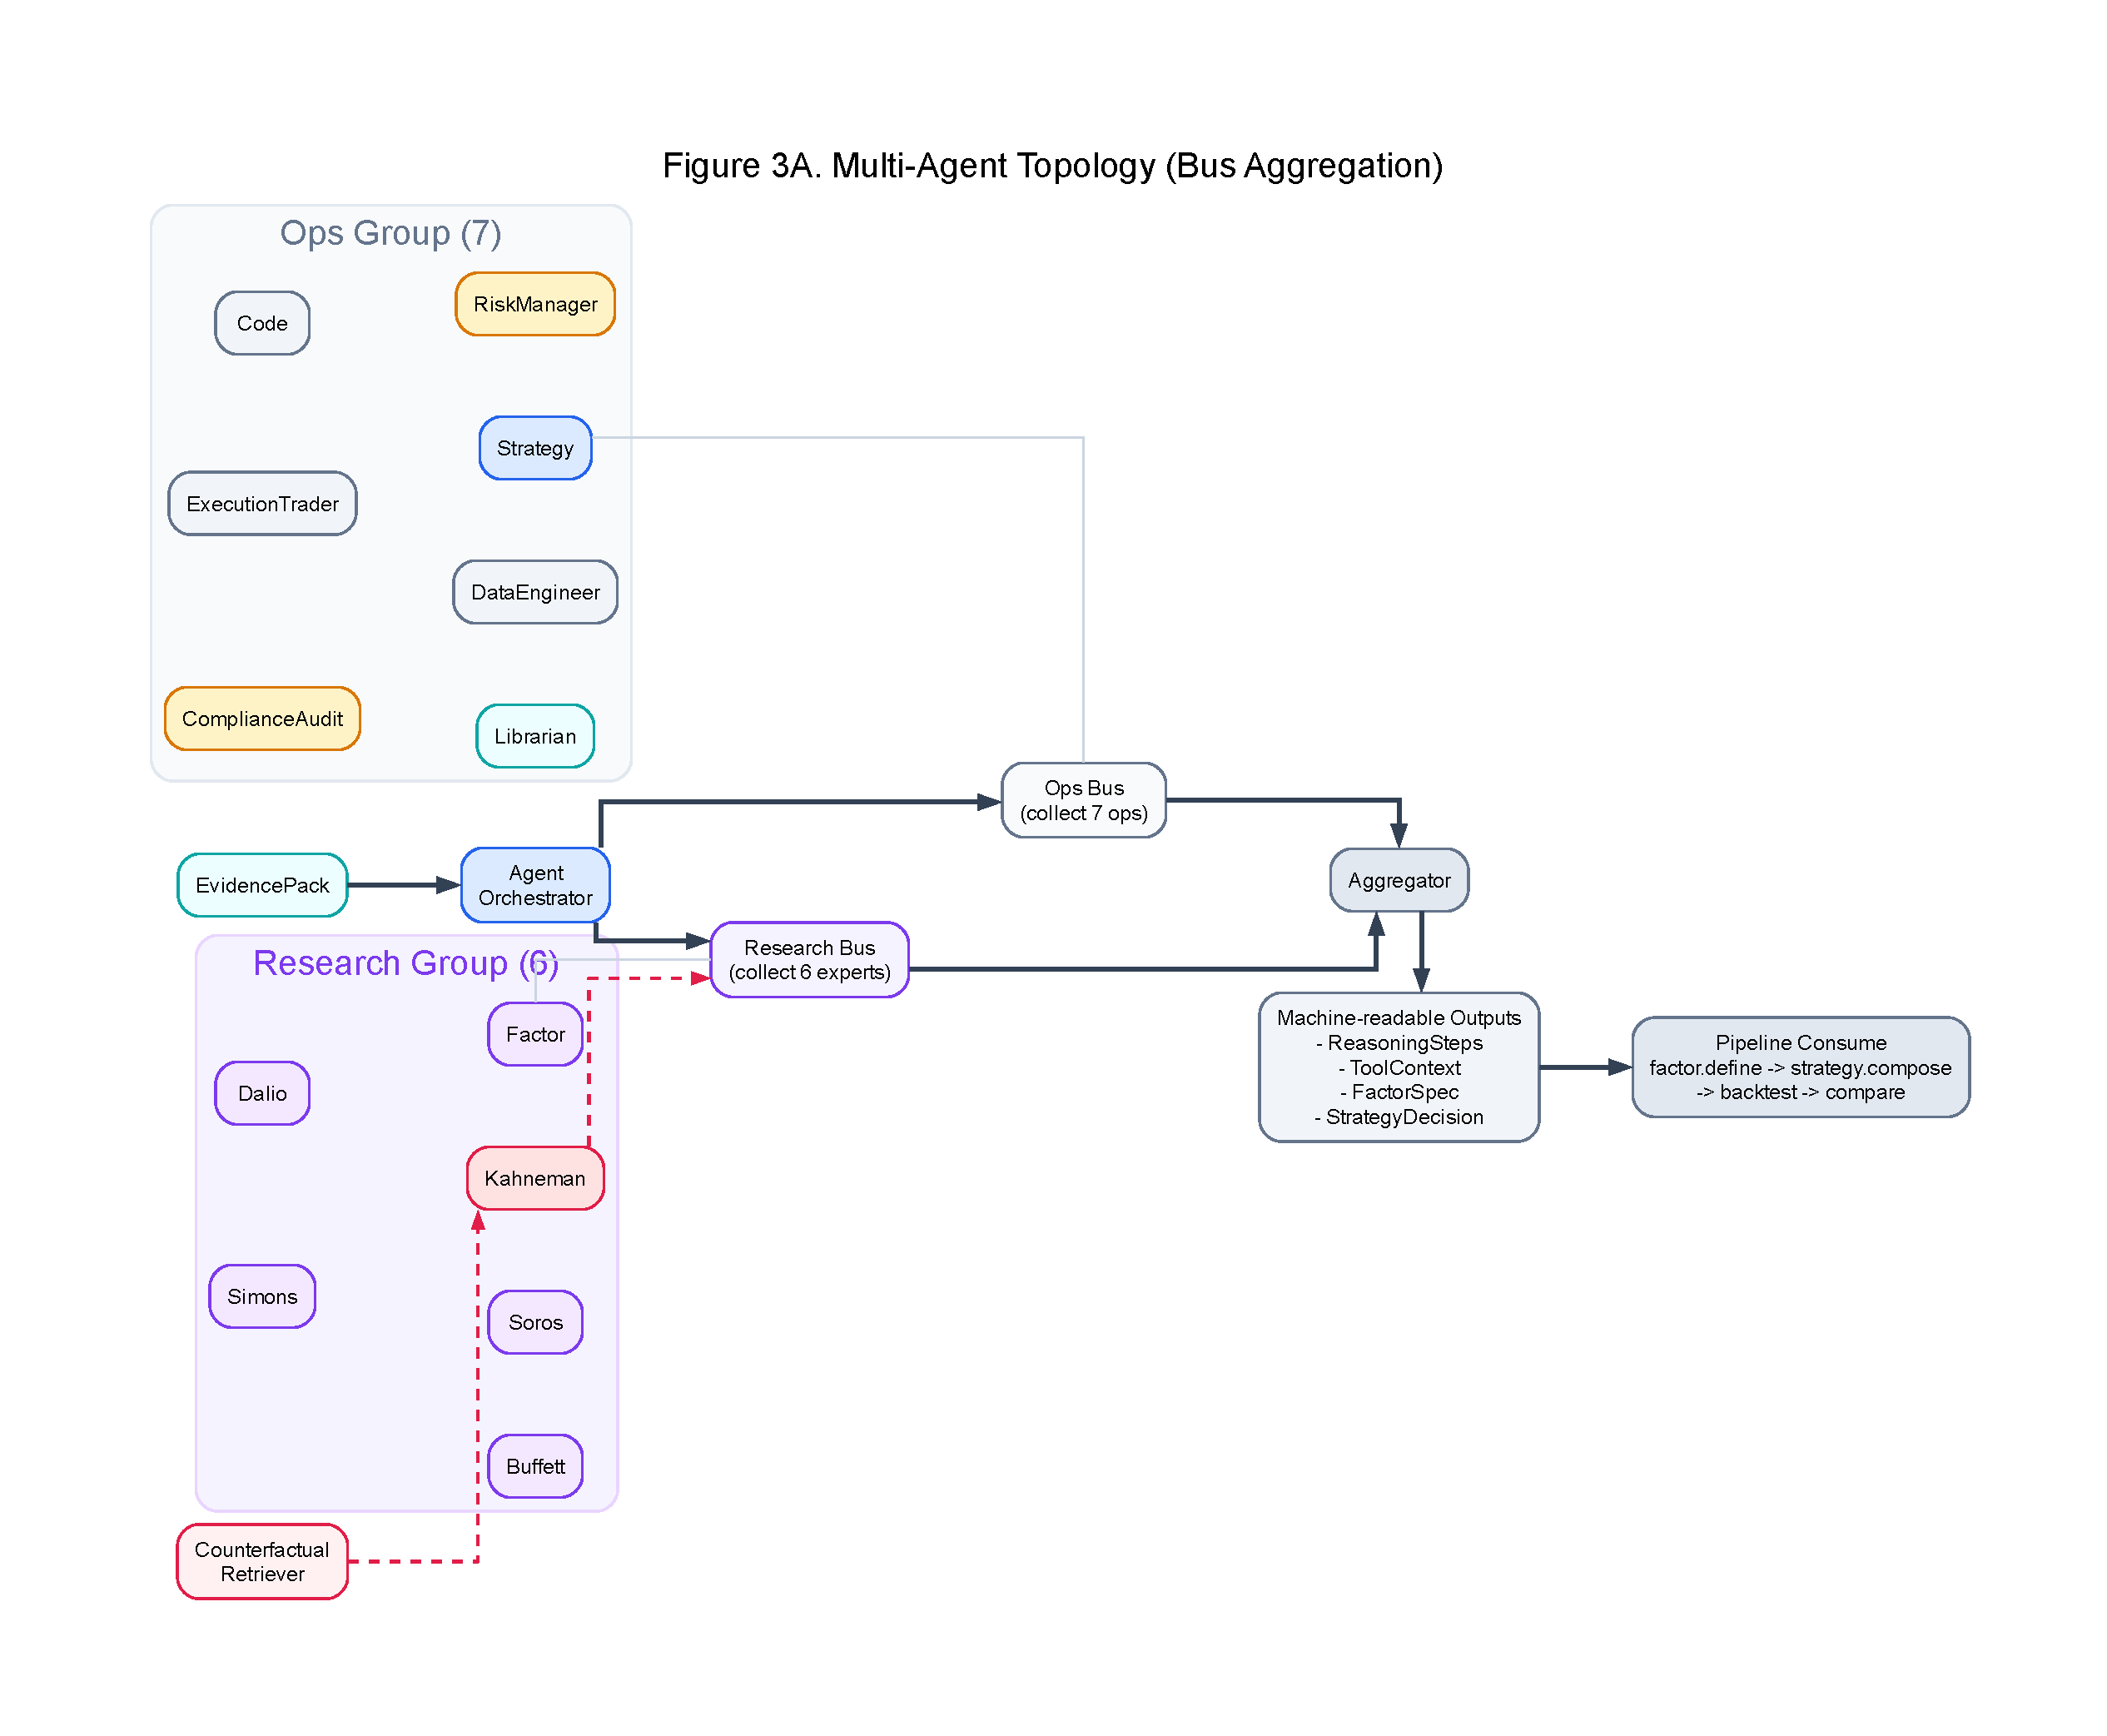
\includegraphics[width=\textwidth]{docs/figures/fig3a_multi_agent_topology.pdf}
\caption{Multi-agent topology with bus aggregation and counterfactual path. 图注（中文）：13 个智能体按 Research/Ops 分组，经由总线汇聚到聚合器并输出可消费工件，突出 Kahneman 反证路径。}
\label{fig:agent-collaboration}
\end{figure*}

\subsection{协作规则（读者可复述版本）}
在同一证据包下，Research 组给出“研究结论与反证后修正”，Ops 组给出“执行与治理约束”。Aggregator 不输出自由文本，而输出机器可消费对象（\tok{ReasoningSteps}、\tok{ToolContext}、\tok{FactorSpec}、\tok{StrategyDecision}），再由 Pipeline 消费执行。这个设计直接避免“看起来合理但无法落地”的结论。

\begin{verifybox}
\footnotesize
\begin{tabularx}{\linewidth}{@{}>{\bfseries}p{1.9cm}X@{}}
UI: & Chat Developer Mode（看推理步骤）；Reports（看候选与选优）；Tasks（看阶段） \\
Artifacts: & \tok{reasoning_steps}、\tok{tool_context}、\tok{strategy_decision} \\
Events: & \tok{reasoning.step.created}、\tok{reasoning.step.updated}、\tok{reasoning.trace.final} \\
\end{tabularx}
\end{verifybox}

\section{因子与策略构建及评估机制}
\subsection{因子从哪里来：从候选到 FactorSpec}
因子不是由单个智能体“拍脑袋命名”，而是由三类输入共同约束。第一类输入来自 \tok{plan.signals}，它规定研究方向；第二类输入来自 \tok{evidence.topics}，它提供事实锚点；第三类输入来自 \tok{dataset.fields}，它限制可计算边界。只有当这三者能闭合成同一命题时，FactorAgent 才会把叙事升级为 \tok{FactorSpec}，并交给 FactorEngine 生成带版本号的 \tok{factor_version}。

贯穿示例里，“波动抬升 + 流动性重定价”先被抽象成“高波动环境下，短期收益信号需被流动性惩罚修正”的假设，再落为可计算式：
\[
\mathrm{score}_t=z(\mathrm{ret}_{20d})-0.6\,z(\mathrm{vol}_{20d})-0.4\,z(\mathrm{illiq}_{20d}) .
\]
\tok{FactorSpec} 的每个字段都对应一个不可省略的决策点。\tok{inputs} 声明字段来源，避免隐藏数据泄露；\tok{transforms} 固化去极值、标准化、行业中性化，使横截面分数可比；\tok{validation_plan} 把“可用”定义成门槛而非印象；\tok{failure_conditions} 提前声明在 JP 高波动且成交深度骤降时应降权或停用；\tok{cost_sensitivity} 则回答“成本上升后净优势还能否保留”。因此，\tok{FactorSpec} 不只是参数容器，而是把研究假设变成可复核实验协议的关键对象。

\subsection{因子如何验证：读者可理解的五个指标}
\paragraph{IC 与 RankIC}
它们回答的是“排序有没有方向感”。直觉上可以把它理解为“每次把股票按因子分数排队，前排是否更常跑赢后排”；在报告中通常读取 \tok{ic_mean} 与 \tok{rank_ic_mean} 的区间稳定性，而不是某一天的峰值。常见误判是把短窗口偶然高值当成长期能力，因此系统会要求跨窗口稳定且样本外不反号。

\paragraph{Decay}
Decay 回答“这条信号能保鲜多久”。如果衰减曲线在 1--2 日就贴近零，说明优势极短，交易成本可能比信号收益增长更快；因此报告不仅显示衰减快慢，也用它约束持有期和调仓频率。很多失败策略并非“方向错”，而是“正确得太短”，这正是 Decay 在策略层的作用。

\paragraph{样本外退化（OOS）}
样本外检验回答“换一段市场还能不能成立”。报告里的 \tok{oos_gap} 直接衡量样本内外落差，落差过大时系统不会把该因子作为单因子主驱动，只允许它作为辅助暴露。这样做是为了避免“回看历史很漂亮，进入新阶段即失效”的典型过拟合。

\paragraph{Sensitivity 与失效条件}
Sensitivity 检查“参数轻微变化时结果是否剧烈抖动”，失效条件检查“哪些情境下应主动不信任该因子”。前者防止把偶然最优参数误当稳定规律，后者防止把风险事件解释成暂时噪声。两者都会写入 \tok{failure_flags} 并传给 StrategyAgent，成为策略层过滤候选的硬信息。

\paragraph{体检结果如何进入策略层}
StrategyAgent 接收的不是一句“因子可用”，而是完整字段：\tok{ic_mean}、\tok{rank_ic_mean}、\tok{decay}、\tok{oos_gap}、\tok{sensitivity}、\tok{failure_flags}、\tok{cost_sensitivity}。这意味着策略生成从一开始就受统计稳定性和交易可实现性共同约束，无法绕开验证环节直接给出“漂亮方案”。

\subsection{策略如何产生并评估选优}
StrategyAgent 的目标不是“写一段交易建议”，而是生成可计算的 \tok{StrategyDecision}。该对象至少包含 \tok{candidates[A,B]}、\tok{selected}、\tok{tradeoff_summary} 与 \tok{why_not_selected}，并与输入因子版本一一对应。候选 A 与 B 常对应两类风格：A 压低换手与回撤，B 提高信号响应速度；二者在同一风险预算下竞争，任何一方被淘汰都要留下可复核理由。

系统的决策函数采用约束下多目标比较，而非“Sharpe 最大即最优”。可写成
\[
J_k=\alpha D_k-\beta T_k-\gamma C_k+\delta R_k,\quad k\in\{A,B\}.
\]
并在 \(\max_{k\in\{A,B\}} J_k\) 的同时满足 \tok{max_drawdown}、\tok{turnover_cap} 与市场执行约束。这个形式的含义是：收益质量、回撤控制、成本脆弱性和情境稳健性必须同时达标，任何单项极优都不能掩盖其他维度的失败。

在贯穿示例中，候选 B 在基准样本的收益指标略高，但 \tok{cost_x2} 与高波动场景下的 \tok{robustness_matrix} 显示其回撤和换手迅速恶化；候选 A 虽然收益略低，却保持更稳的最坏情境表现，因此最终被选为 \tok{selected}，并在 B 的记录中填入 \tok{why_not_selected}，其值为“cost-drawdown fragile”。回测后并不直接结束，MetaRunner 还会把 A/B 的账本与稳健性结果回灌到比较器，避免“基准样本领先即定案”的单次误判。

\subsection{Algorithm 1：Variant Execution Loop}
\begin{algorithm}[t]
\caption{Variant Execution Loop (Factor $\rightarrow$ Strategy $\rightarrow$ Backtest)}
\begin{algorithmic}[1]
\STATE Receive \tok{plan}, \tok{dataset_version}, \tok{evidence_pack}
\FOR{each \tok{variant} in experiment matrix}
  \STATE Build \tok{FactorSpec}; derive \tok{factor_version}
  \STATE Run factor engine; produce \tok{FactorReport}
  \STATE Generate strategy candidates (A/B); select one with \tok{why_not_selected}
  \STATE Build \tok{BacktestRequest} with lineage fields and constraints
  \STATE Run backtest; persist \tok{run_id}, metrics, diagnostics
\ENDFOR
\STATE Compare variants; output best report and robustness summary
\end{algorithmic}
\end{algorithm}
\noindent\textbf{中文解释：}算法只定义执行顺序；真正的“可解释选优”由 4.1--4.3 的字段约束与报告检查完成。

\subsection{Algorithm 2：Strategy Selection with Trade-off}
\begin{algorithm}[t]
\caption{Strategy Selection with Trade-off (A/B + why\_not\_selected)}
\begin{algorithmic}[1]
\STATE Input factor health, market rules, risk budget, and constraints
\STATE Construct Candidate A and Candidate B
\STATE Score each candidate on drawdown control, cost, and regime robustness
\IF{A wins}
  \STATE Set selected = A; set B.\tok{why_not_selected}
\ELSE
  \STATE Set selected = B; set A.\tok{why_not_selected}
\ENDIF
\STATE Emit \tok{StrategyDecision} with selected rationale and trade-off summary
\end{algorithmic}
\end{algorithm}
\noindent\textbf{中文解释：}该算法避免“只给结论不给对照”，并强制保留 \tok{why_not_selected} 供审计复核。

\subsection{Artifacts \& Lineage（工件及血缘）}
\begin{table*}[t]
\centering
\scriptsize
\setlength{\tabcolsep}{4pt}
\begin{tabularx}{\textwidth}{p{2.2cm}p{3.9cm}p{2.4cm}p{2.7cm}X}
\toprule
工件 & 关键字段（示例） & 生成阶段 & 存储位置 & 页面查看 \\
\midrule
EvidencePack & \tok{evidence_pack_id}, \tok{sources[]}, \tok{timestamp}, \tok{credibility} & evidence.pack & Registry + evidence \mbox{artifacts} & Evidence / Chat(Dev) \\
FactorSpec & \tok{factor_id/version}, \tok{inputs}, \tok{transforms}, \tok{validation_plan}, \tok{failure_conditions}, \tok{cost_sensitivity} & factor.define & Registry + factor artifacts & Factors / Reports \\
FactorReport & \tok{ic_mean}, \tok{rank_ic_mean}, \tok{decay}, \tok{oos_gap}, \tok{sensitivity} & factor.define & Artifact files + run context & Factors / Reports \\
StrategyDecision & \tok{candidates}, \tok{selected}, \tok{tradeoff_summary}, \tok{why_not_selected} & strategy.compose & Run registry payload & Reports \\
BacktestRequest & \tok{dataset_version}, \tok{factor_versions}, \tok{strategy_decision}, \tok{constraints}, \tok{evidence_refs} & variant.backtest & Registry requests & Tasks / Reports \\
BacktestReport & \tok{run_id}, \tok{metrics}, \tok{cost_breakdown}, \tok{attribution}, \tok{diagnostics} & backtest.compare & runs registry + \mbox{artifacts} & Reports \\
Robustness\\Report & stress \mbox{matrix}, worst-case summary, variant table & robustness.compare & Run registry + \mbox{artifacts} & Reports \\
\bottomrule
\end{tabularx}
\caption{表1：Artifacts \& Lineage（工件及血缘）。读者可用该表回答“每个结论从哪里来，最终存在哪里，去哪一页看”。}
\label{tab:artifacts-lineage}
\end{table*}

\begin{table*}[t]
\centering
\scriptsize
\setlength{\tabcolsep}{4pt}
\begin{tabularx}{\textwidth}{p{1.7cm}p{3.2cm}p{3.2cm}p{3.2cm}X}
\toprule
页面 & 主要任务 & 典型输入 & 典型输出 & 关联工件 \\
\midrule
Chat & 提问、改约束、触发任务、查看推理步骤 & question, constraints & plan trigger, live reasoning stream & EvidencePack, ReasoningSteps, trace\_id \\
Pipeline & 查看阶段计划、预检、运行进度 & plan\_id, stage status & stage summaries, artifact links & Plan, FactorSpec, StrategyDecision \\
Tasks & 追踪父子任务与心跳 & task\_id / parent task & stage timeline, retries, child runs & BacktestRequest, run\_id \\
Reports & 查看结果、候选对比、归因与成本 & run\_id & metrics, robustness \mbox{matrix}, selected rationale & BacktestReport, StrategyDecision \\
Evidence & 核验证据来源与时间一致性 & evidence\_pack\_id & source \mbox{title}/ts/snippet/credibility & EvidencePack \\
Risk & 审批、门控、风险解释 & run\_id, risk policy & approve/reject, gate \mbox{explanation} & BacktestReport, constraints, trace\_id \\
Settings & 配置默认约束与开发开关 & system policy & policy snapshot, mode config & constraints templates, audit defaults \\
\bottomrule
\end{tabularx}
\caption{表2：UI Pages \& What You Do There。页面职责与工件绑定关系用于支撑跨页复核。}
\label{tab:ui-workflow}
\end{table*}

\begin{verifybox}
\footnotesize
\begin{tabularx}{\linewidth}{@{}>{\bfseries}p{1.9cm}X@{}}
UI: & \tok{/factors}、\tok{/reports/{runId}}、\tok{/tasks} \\
Artifacts: & \tok{FactorSpec}、\tok{FactorReport}、\tok{StrategyDecision}、\tok{BacktestReport} \\
Events: & \tok{task.variant_started}、\tok{task.progress}、\tok{task.variant_done} \\
\end{tabularx}
\end{verifybox}

\section{可解释性实现}
\subsection{三种解释性输出：它们各自解决什么质疑}
Evidence traceability 直接回应“你是不是在编故事”。在 OpenFinance 中，任何结论句都应回指 \tok{evidence_refs}，并能在 Evidence 页看到 \tok{source_title}、\tok{source_ts}、\tok{source_snippet}、\tok{credibility_breakdown}。如果这些字段缺失，结论就无法区分“有来源的判断”和“语言上通顺的猜测”。

Reasoning visibility 回应“系统是否跳步得出结论”。平台不公开私有链式思维，但会公开 \tok{reasoning_steps}、\tok{evidence_refs} 与 \tok{confidence_delta}，让读者看到每一步证据引用和置信度变化。这样既避免泄露内部推理细节，也给出足够证据证明结论来自逐步推导而非一次性生成。

Reproducibility 回应“同条件下能否重放同一路径”。每次运行都会绑定 \tok{trace_id}，并把计划、证据、因子、策略、回测和审批串成可恢复链路；只要上下文一致，复盘者就能在同一入口重建同一执行过程。没有这层机制，报告只能被阅读，不能被反驳或复现。

\subsection{UI 路径与字段：要验证什么就去哪里、看到什么}
如果要验证“结论是否有证据”，入口是 Evidence 页：应先看 \tok{source_type}，区分 \tok{mock} 与 \tok{local_corpus}，再看 \tok{source_title}、\tok{source_ts} 和 \tok{credibility_breakdown} 是否支持该结论。若证据时间滞后或可信度拆解缺失，结论就应被降级为待核验而非可执行建议。

如果要验证“推理是否逐步形成”，入口是 Chat Dev Mode：应看到 \tok{reasoning.step.created} 按时间流入，而不是任务结束后一次性回填。重点字段是 \tok{step_type}、\tok{evidence_refs}、\tok{confidence_delta}；只要出现“结论先到、证据后补”，就说明链路有断层。

如果要验证“选优是否可复核”，入口是 Reports 页：应同时看到 \tok{factor_versions}、\tok{candidates}、\tok{why_not_selected}、\tok{cost_breakdown} 与 \tok{robustness_matrix}。这组字段能够回答“为何选 A 不选 B”，并暴露是否存在“只看基准 Sharpe”导致的误选。

如果要验证“系统是否真实跑完而非假死”，入口是 Tasks 与 Risk 页：Tasks 需显示 \tok{parent_task}、\tok{child_tasks}、\tok{heartbeat_stage}、\tok{artifact_links}，Risk 需显示门禁结论与审批理由。两页结合后，读者可以区分“任务仍在运行”“任务异常重试”和“审批拒绝”这三种状态。

\subsection{回放与复盘}
当结果需要复盘时，使用 \url{/trace/\{trace_id\}/restore} 恢复上下文，再按“Evidence $\rightarrow$ Reasoning Steps $\rightarrow$ Report $\rightarrow$ Risk”路径逐层核验。该机制确保“结论、过程、约束”三者在一次复盘中可以闭环对齐。

\begin{verifybox}
\footnotesize
\begin{tabularx}{\linewidth}{@{}>{\bfseries}p{1.9cm}X@{}}
UI: & Evidence / Chat(Dev) / Reports / Tasks / Risk \\
Artifacts: & \tok{evidence_pack}、\tok{reasoning_steps}、\tok{factor_versions}、\tok{strategy_decision}、\tok{trace_id} \\
Events: & \tok{reasoning.step.*}、\tok{reasoning.trace.final}、\tok{audit.trace} \\
\end{tabularx}
\end{verifybox}

\section{当前范围与限制}
\textbf{(1) 数据边界}：当前系统支持 mock 与本地语料并行，二者在覆盖率、时效性、缺失值模式上可能不同。若把 mock 条件下通过的因子直接外推到真实市场，常见后果是信号稳定性被高估。上线前需要对 \tok{dataset_version} 与 \tok{source_type} 做分层回归验证。\\
\textbf{(2) 统计边界}：IC 为正并不保证可交易，样本外退化、策略拥挤与成本冲击会显著改变排名。尤其在高换手候选中，“基准 Sharpe 最优”常在成本翻倍情境下失效，因此必须把 robustness 作为选优前置门槛。\\
\textbf{(3) 系统边界}：事件流可能出现丢失或延迟，任务可能因外部依赖中断，\tok{market_context} 锁定错误会导致策略在错误市场规则下评估。虽然系统提供 heartbeat、重试与 \tok{trace_restore}，但这些机制只能降低故障影响，不能替代运行时监控与人工复核。

\section{结论}
本文在不改变章节主结构与图号的前提下，完成了 OpenFinance 草稿的第二轮打磨：图示从“模块堆叠”改为“主线可复述”；方法从“代码片段”改为“伪代码 + 对象表 + 血缘表”；叙事从“局部说明”改为“贯穿示例闭环”。其核心价值不在于单一算法，而在于让系统运行、智能体协作、因子策略构建与可解释复核形成同一条可执行、可审计、可回放链路。

\section*{影响声明}
本工作旨在提升量化研究流程透明度与安全性。潜在风险在于用户忽略审批与风险门控，或将模拟结果误解为实盘保证。系统默认关闭 live trading，并提供审批状态机、kill switch、风险事件流与可恢复审计链路。

\bibliography{openfinance_refs}
\bibliographystyle{icml2026}

\end{document}
